\chapter{Radioactive Half-Life}

%TODO add instructor note: to close door to KPTC 003, need to toggle switch that keeps it open, which is above the door.

The physical laws of radioactivity predict that the rate of decay (number of atoms
decayed / time interval) is proportional to the number of radioactive nuclei present. This
is due to the independence of the decay of
each atom in the sample. The proportionality constant that describes the decay rate
depends on the specific radioactive nucleus. A concise and suggestive way to
characterize the nucleus is by its half-life, the time it takes for the number of radioactive
nuclei to decrease to half of the initial value. You will obtain data to check the form of
the law and to determine the half-life of one or more isotopes of silver.

We will use a device known as a neutron ``Howitzer''. It consists of a source of alpha
particles and a material that absorbs alpha particles and immediately decays by emitting
neutrons. (The neutrons shoot out from the barrel of the shielded volume, vaguely like
shells from WWI artillery, hence the name.)

\subsection{Scientific Background}

Nuclear reactions play an important role in astronomy, geophysical sciences, archaeology, and physical anthropology. They explain energy generation in stars, the relative abundance of chemical elements, and provide a method for determining the age of things --- from a piece of wood, to a meteorite, to the universe itself.

Most elements exist in a number of different forms, called isotopes, some of which are unstable and can change from one type of element to another. When this occurs, a high-energy particle is usually emitted from the nucleus of the element as it changes. By measuring the ratios of isotopes with differing decay rates, one can infer the age of an object.

\section{The irradiation process}

We will let the neutrons bombard a small sample of the stable isotope of silver, $^{107}$Ag, to
produce $^{108}$Ag, via the reaction
\begin{equation}
 ^{107}\textrm{Ag} + \mathrm{n} \rightarrow\, ^{108}\textrm{Ag} + \gamma \,,
\end{equation}
where $\mathrm{n}$ represents a neutron and $\gamma$ a gamma particle --- that is, a high energy photon.

The radioactive isotope of silver, $^{108}$Ag, spontaneously decays to an isotope of cadmium
with the same mass number, $^{108}$Cd, by the reaction
\begin{equation}
 ^{108}\textrm{Ag} \rightarrow\, ^{108}\textrm{Cd} + \mathrm{e}^- + \gamma \,,
\end{equation}
where $\mathrm{e}^-$ is an electron (that is, a $\beta$ particle, as we saw and measured last week).

Your TA will bombard silver foils with neutrons using the neutron howitzer. Some of the
nuclei in the foil will have captured a neutron and transformed into a different isotope
which is unstable and can be detected via their decay products. Each group will be given
one of these silver foils.

\section{The neutron source}

The source is a mixture of plutonium and beryllium. The plutonium decays via alpha emission and the beryllium absorbs the alpha to become carbon + a free neutron. The neutron has an energy given by a very complicated distribution, but the energy distribution goes up to $\sim 11\:$MeV. The paraffin shielding (and the lucite in the plug) slows down neutrons, so that anything which escapes is thermalized such that $E \sim kT \sim 1/40\:$eV. At the point where the foils are placed, the neutrons have been slowed some, but not completely... if they are a full 11 MeV still, they are too energetic to bind with the silver, so the foils are absorbing from the lower end of the spectrum or from neutrons that have scattered enough material to have less energy than they started with.

The activity of the Pu-Be core is an astounding 5 Ci (!!), but that's the alpha flux which doesn't penetrate out of the core. The neutron flux is considerably less. There is about 80 g of plutonium mixed with 41 g of beryllium and a listed, unshielded emission rate of $9 \times 10^6\:$n/sec.

\begin{framed}
	\textbf{Warning: Radioactive Material!} The radiation levels are very low and they present no hazard for the short time that you are in the lab. We estimate that you will receive an additional dose of ionizing radiation that is much less than what you receive every day normally. You can compare this to the example doses in Fig.~\ref{rad1:doses}. Here are tips to keep your exposure low:
	\begin{itemize}
		\item \textbf{Do not have any food, drink, food containers, or make-up on the lab bench, and do not consume any food or drink, and do not apply cosmetics, in the lab.}
		
		\item \textbf{Decrease time with and increase distance from sources.} Handle the silver foils only when you need to be for the lab.
	\end{itemize}
\end{framed}

\begin{framed}
	\textbf{Caution: Fragile Equipment!} The Geiger tube (the upright cylinder sitting in the plastic stand and connected to a coaxial cable at the top) hold a gas under vacuum, with a thin, fragile window at the bottom of the tube. Do not touch it, as it breaks extremely easily.
\end{framed}

\begin{figure}
	\centering
	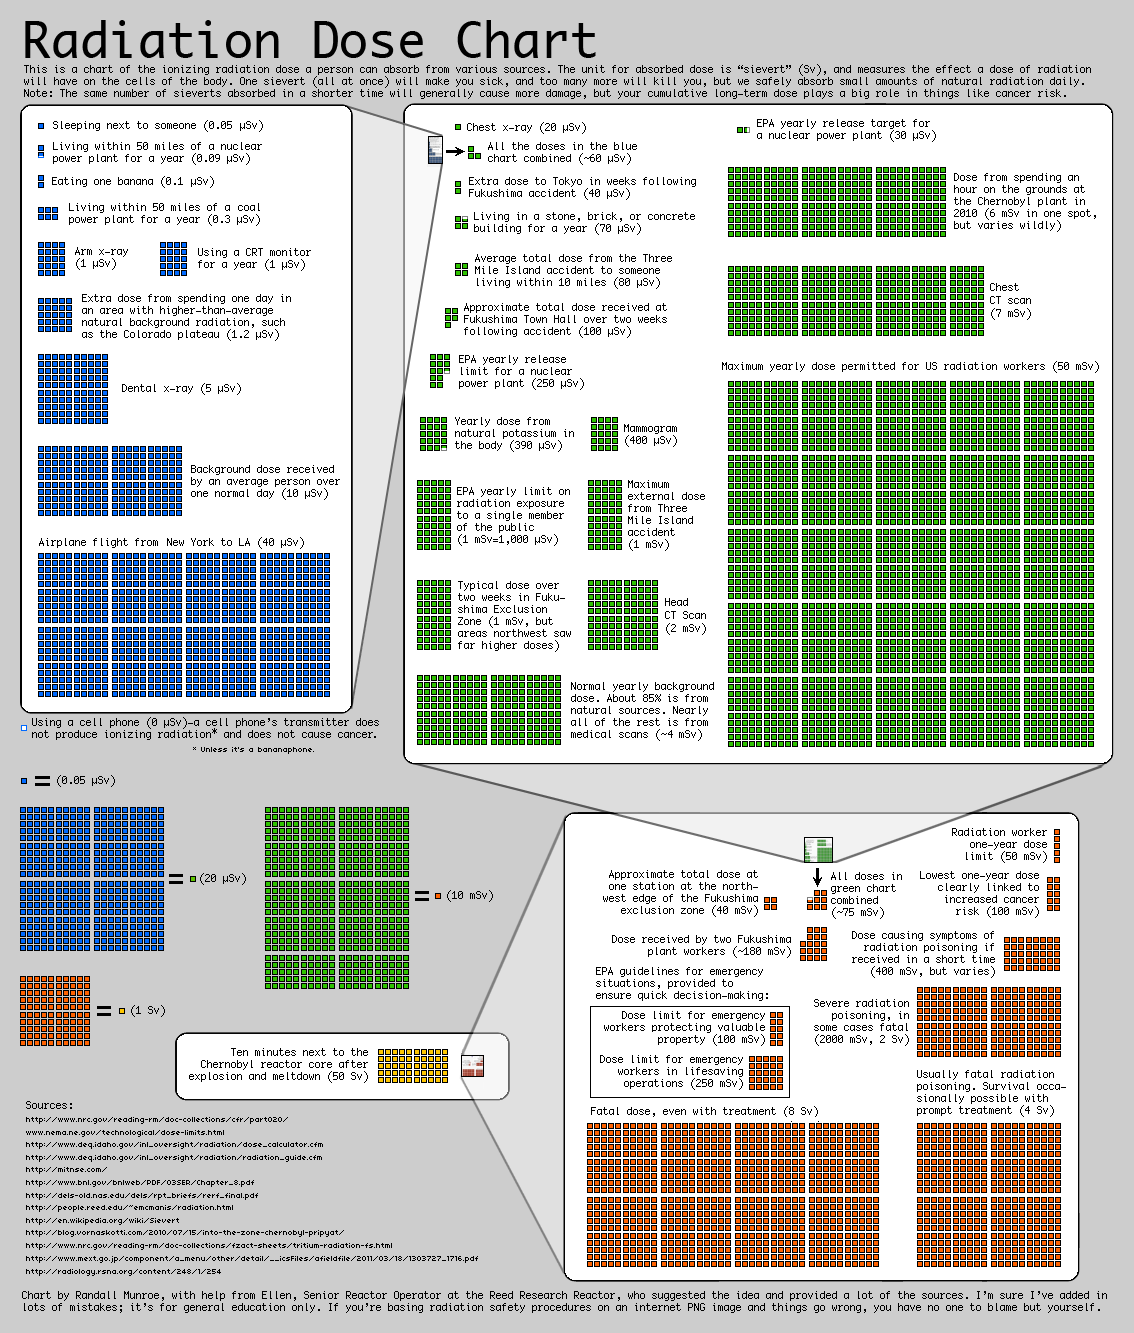
\includegraphics[width=\textwidth]{radioactivity-1/radiation-xkcd}
	\caption{A chart of ionizing radiation dose from various sources. Source: \url{https://xkcd.com/radiation/}}\label{rad1:doses}
\end{figure}

\subsection{Theory of counting statistics}

If you've ever worked in a not-too-busy retail environment, you’ve probably had the
experience of realizing (perhaps) that random and uniform are two quite different things.
You no doubt have sat waiting for customers, with nobody around for long stretches of
time, and then, as though they'd coordinated in advance, a half dozen people all show up
within a few minutes of each other. Each customer is indeed independent (no, they didn't
have a Twitter call to organize a flashmob!\footnote{Yes, popular interest in flash mobs peaked in 2011. Bear with us here.}) yet their arrival times clearly appear clustered. They are, in fact. But randomly. Uniform – one customer each minute – is quite dramatically different than a random procedure that yields one customer per minute on average. Retail customers (to a great extent), and elementary particles, act randomly, not uniformly.

Each atom in a radioactive sample has, per unit time, some probability of undergoing
radioactive decay. That probability is independent of all the other atoms in the sample.
Each atom decays, or not, based on its own probability and no other. The ensemble of
particle decay counts that one would measure in the sample (using a Geiger counter as we will
do, for example) is described by the something called the Poisson distribution, which
gives, in this instance, the probability of a integer number of events occurring in a fixed
interval of time, given an average rate. For large count rates, like we have here, the
Poisson distribution is indistinguishable from the normal distribution (that is, a simple
Gaussian function).

Specifically, for a process that produces an average $\bar{N}$ counts in a certain time duration (in the case of large $N$), the expected measurement of that count for that time duration is a
random draw from a normal distribution with mean $\bar{N}$ and a standard deviation of
$\sqrt{N}$.

\begin{framed}
	\textbf{The Apparatus.}
	
	The energetic particles produced in radioactive decay reactions can be detected by a
	device called a Geiger counter. This consists of a tube filled with inert gas with a wire
	running through it. A high voltage is applied between the wire and the tube. When a high-
	energy particle enters the tube, it can ionize the gas. The freed electrons produce a brief
	pulse of current at the output of the device. The pulses can then be counted.
	
	The counter itself is controlled using buttons on the front panel. \texttt{COUNT} begins the count
	and starts the timer, \texttt{STOP} pauses the count and timer, and \texttt{RESET} sets the count and
	timer to zero. Use the dial on the counter to change the display between the count and the
	elapsed time. When you first turn on the Geiger counter you need to set the voltage to
	$1000\:$V --- the TA will demonstrate how. \textbf{Caution:} Do not turn off the voltage during the
	experiment; use the \texttt{STOP} button to stop the count. \textbf{Do not touch the window on the
		bottom of the tube, as it breaks extremely easily.}
\end{framed}

\section{Procedure}

Your task is to measure the half-life of $^{108}$Ag. We will use the Geiger tube to count
decays. That is, we will count the $\beta$ particles --- the gamma rays make only a small
contribution to the counts in this instance. You should attempt to carry out the counting
fairly quickly after the silver foil is removed from the howitzer as the decay time is quite
short.

\begin{steps}
	\item Before the neutron irradiation begins you will want to record the background rate. Press
\texttt{STOP} and \texttt{RESET} on the counter to set the display to zero.

	\item Next, press \texttt{COUNT} with no
sample below the Geiger tube and collect the total number of background counts, $N_\textrm{bkg}$ ,
that accumulate in approximately 5 minutes. Once 5 minutes has elapsed press \texttt{STOP} to
end the count.

	\item Turn the dial to \texttt{TIME} and record a precise measurement of the elapsed
time, $t$, in seconds. The background rate $R_\textrm{bkg}$ is found with
\begin{equation}
R_\textrm{bkg} = N_\textrm{bkg} /t
\end{equation}
with an uncertainty given by Poisson statistics. \textbf{Report both the background rate and uncertainty in your lab report.}

	\item While the samples are being irradiated, set up your measurement apparatus.

	\item Once the samples are ready, quickly place a silver foil sample in the tray below the Geiger tube. Using a stopwatch and the counter, record the number of counts and the time at 30 second intervals for about 10 minutes, continuously.%
%Unlike last week's lab with the same apparatus, you will be recording data continuously, and so
You will need to use the watch to record times rather
than timer built into the Geiger counter. \textbf{Record your data.} \textit{You may want to take a video of the stopwatch and counter to get more precise readings of the 30-second intervals.}
\end{steps}


\section{Calculations}

The experimental data will be used to determine a half-life (or half-lives). We know that
the decay rate ($R=\Delta N / \Delta t$) of a radioactive nuclide is proportional to the number of nuclei present. The proportionality constant is called the decay constant $\lambda$, and the equation that describes what was just discussed is
\begin{equation}
 R = \lambda N \,,
\end{equation}
where $N$ is the background-subtracted counts. Using integral calculus and the above equation, we find
\begin{equation}
 \frac{N}{N_0} = e^{-\lambda t} \,,
\end{equation}
where $N_0$ is the number of nuclei at the initial time $t=0$. The half life $T_{1/2}$ is defined by
the time it takes for $N = N_0 /2$ and is related to the decay constant by $T_{1/2} = \ln(2)/ \lambda$, where
$\ln()$ is the natural logarithm function, and so $\ln(2) \approx 0.693$.

We can now write the radioactive decay equation as
\begin{equation}
 R = \lambda N_0 e^{-t \ln(2) / T_{1/2}} \,.
\end{equation}
Taking the logarithm of both sides and substituting for $N$ gives
\begin{equation}
 \ln(R) = - \left(\frac{\ln(2)}{T_{1/2}} \right) t + \mathrm{const} \,.
\end{equation}
Your TA will help you to understand the details of this derivation.

\begin{steps}
	\item Make a plot showing $\ln(R)$ on the vertical axis and elapsed time, $t$, along the horizontal axis. Don’t forget to subtract the background where appropriate.

	\item Calculate the slope and use this value to solve for the half life using the above equations. \textbf{Report this value along with a table of your decay rate data and the plot described above.}
\end{steps}

\section{Questions (these should be included in your lab report)}

\begin{steps}
	\item Look up the half-lives of the various nuclides of silver. What is the published
	half-life of the nuclide you’re observing? How does this compare with your
	calculated result? Calculate the percent difference in your result.
	
	\item For the silver foil, how long would it take before you would expect to detect only
	one count per second, background corrected?
	
	\item The detector only measures particles that travel up into the detector. The majority
	of particles traveling in the other directions escape detection. Will this short-
	coming affect the measured half-life? If so, how? If not, why not?
	
	\item Describe one thing you could change in this experiment that could lead to a more
	accurate measurement of the half-life of the silver isotope.
	
	\item The particular irradiated silver sample you used contained some unknown
	percentage of the unstable silver isotope, and was irradiated at some unmeasured
	time before you began your experiment. Does this matter to your results? Explain.
	
\end{steps}

\section{Report checklist and grading}

Each item below is worth 10 points, and there is an additional 10 points for attendance and participation.

\begin{enumerate}
	\item Background rate and uncertainty (Step 3)
	
	\item Plot of $\ln(R)$ vs.\ $t$ with the trendline and equation listed. (Step 6)
	
	\item Calculation of slope of above plot and work of solving for the half-life, with the final half-life determination. (Step 7)
	
	\item Answers to questions in Steps 8--9.
	
	\item Answers to questions in Steps 10--12.
\end{enumerate}